\documentclass[11pt]{article}

% This package sets the margins to 1in
\usepackage{fullpage}
\usepackage{graphicx}
\usepackage{multicol}

\title{Project 2}
\author{Bill Collins and Alec Gerhart}
\date{April 29, 2016}
\begin{document}
\begin{multicols}{2}

\maketitle


\center 
Abstract
\flushleft
For our project, we created a 50x50 grid representing a world, where agents exist. In this world, the agents find food to survive, while also procreating. The goal was to see what changes implementing evolution would have, rather than letting future generations just have random attributes. We could see changes occurring with evolution, but in the end, the goal became keeping the population alive, which we were unfortunately unable to do.
\center 
Problem Description 
\flushleft

Predicting the growth and depletion of a population has been important in keeping societies alive. In most governments today, populations are regularly checked to update the state of a nation. The goal of our next-event simulation is to create a virtual population on a 50x50 grid that can feed and reproduce so that we can find patterns in how a society can sustain itself. This will allow us to see limits in population growth and decay, and may allow us to find an average amount of members in the population of this very basic society.


\center 
Validation and Verificaiton
\flushleft
To create our simulation, we first had to create the members of our population. We will refer to these members as agents.

Agents search within their field of view for the location on the grid that has the most food. They travel to this location to pick up the food. If the agent is fertile, it will also look for an agent of the opposite gender to reproduce with. If the agent runs out of food, then it starves to death. If the agent never starves to death, then it will die of old age. \newline

We created an agent class that would represent an agent. The agent's constructor took in the current time (the time that the agent was created), the agent's unique id, and its location on the grid (x and y coordinates). These values were all saved in the agent object, and other values were created within the constructor. The agent has a variable that tells whether or not it is alive, which starts at True. When the agent dies, we set this value to false. The agent's gender is determined by Bernoulli(0.5), where they are male if this value is 1. The agent becomes fertile at a time determined by Uniform(12, 15). If the agent is male, then their fertility ends at Uniform(40, 50). If the agent is female, then fertility ends at Uniform(50, 60). The agent's metabolism, which is how quickly their food decreases, is determined by Uniform(1, 4). The agent loses this amount of food for each unit of time that passes. As stated before, the agent can die of old age. This age is determined by Uniform(60, 100). The agent also has a pregnancy variable, which is true if the agent or its mate is pregnant, and is false otherwise. The agent also has a field of view, which is an Equilikely value between 1 and 6, and represents how far an agent can see.
The agent also starts with wealth, or food-level, of 100.
\newline
Later on, we decided to add evolution to the agents of the simulation. If the agent has parents (it is not part of the first generation), then its attributes are determined by its parents. The age that it hits puberty is a Uniform value between the ages that the parents hit puberty. Its lifespan (how long the agent lives if it does not die of starvation) is a Uniform value between its parents' lifespans. Its field of view is an Equilikely value between its parents' fields of view. Its metabolism is a uniform value between its parents metabolisms.
\newline
To ensure that the agents were working properly, we mainly had to focus on their interactions with the world and other agents. We know that the methods that create their attributes work perfectly fine, as they were given to us by Dr. Coleman. To test their interactions, we had to make sure that their locations were kept properly when moving. When they move to a new location, we had to make sure that they gained the food from the location, and that the amount of food on that location went to 0.\\
The last interaction we had to test was procreation. The only time two agents could procreate is if they are both fertile, not pregnant and have enough food to give to their proposed child. With the knowledge that each agent should start with a wealth of 100, each parent gives half of that 100, and they also need to have enough food to not starve to death before the child is born. Thus, each agent must have at least $50 + 0.75 * metabolism$, in order to have a child (0.75 is the amount of time for pregnancy). Side note, if both agents are having a baby, their time for movement must be pushed back by $0.75$. Once we tested all possible scenarios of agents trying to procreate and we got the expected results, we knew the agents were working properly.
\newline
After this, we created a food object. This object will represent the amount of food that is on a space on the grid. The constructor of this object takes in the maximum capacity that the food object can take. The food object starts with the maximum amount of food and cannot go above this number. When the food is taken, the amount of food goes down to 0. When the food is lower than its maximum capacity, then the amount of food in the object increases by 1 for every unit of time.
\newline
To test the food object, we made sure that food never dropped below zero, and that food grew back at the correct rate (equal to time). For example, if the amount of time that passed is 1.6, then 1.6 food should grow back. We also made sure that the amount food never went past its max capacity. Once this all worked, we moved to the next object.
\newline
After creating the food object, we created a map object to act as the 50x50 grid. This object creates a food object for each box in the grid where the x and y values determine the maximum amount of food with the following functions: \newline
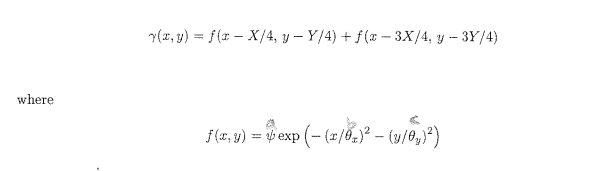
\includegraphics[width=80mm]{MaxFoodFunction.PNG} \newline
which creates the following grid: \newline
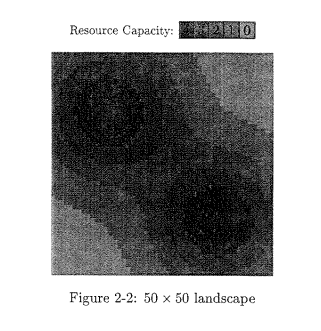
\includegraphics[width=80mm]{ResourceCapacity.PNG} \newline
Testing the map involved making sure that the initial values for each food object inside the map represented the picture above. To make sure that they were creating an outline like the picture, we had to output all the values of the map. Once we saw that the values were higher in the spots where they are darker in that picture, and the spots that had a lighter color to them were lower, we believed the map was working.
\newline
The last object that we created was the event object. This object holds the type of an event, the time that the event takes place in the next-event simulation, and the id of the agent that it relates to. If the type of the event is birth, it also holds the id numbers of the agents that are having the child.
\newline
To test the events, we had to make sure that the events were kept in proper order, in order to avoid having an event occur before it should. This just meant we had to order by their times, when a new event was created, for which we used Python's sorting method to do. Once we knew the ordering was correct, we had to make sure each event did their job. For example, if an event for puberty occurs, we had to make sure the agent that is hitting puberty became fertile. If the event is a movement, we had to make sure the agent's location is changed to the destination, the agent picked up the food, and that the agent's next destination is picked. Another thing that occurs here is checking if any agent is next to this agent. If so, the possibility of having a child must be explored. Once every type of event was working and being scheduled properly, we could move on to writing up the simulation.
\newline

\center 
Experiments and Data
\flushleft

Now that we had written our objects, we were able to create our simulation. We created a simulation method that took in the starting number of agents and the end time of the simulation. The first step of this simulation was to create an event of type ''check'' for every 5 units of time. An event of type ''check'' records the number of agents that are currently alive in the simulation and puts it into a list to be returned later. \newline
After this, we created a list of agents. When creating the agents, we created events for their beginning and end of fertility, as well as their death from old age. These events affect their agents by making them fertile, ending their fertility, and killing them.
\newline
It also creates their first movement event. To do this, we took the agent's feild of view (refer to this as FOV) to find the location with the most food that is within this range. We looked at All of the spots that were FOV steps to the left, right, in front of, and behind the the agent and found the location with the most food. The amount of time that it takes to move to the location is 0.5 + Exponential(0.5) per space. When the agent gets to its desired location, it picks up all of the food and searches to see if a mate is in range. It searches the same way that it searches for food, by looking left, right, forward, and backwards within the range of FOV. If the agent is fertile, and it finds an agent of the opposite gender who is fertile, whose pregnancy variable is false, and who can spare food for a child, then the two agents cannot move for 0.75 time intervals. They're pregnancy variables become true, and each agent needs to give 50 units of food (half of the starting value). An event of type birth is created for 0.75 time intervals after the current time, which creates another agent and the events that go with creating an agent. Then the parent agents' pregnancy variables become false again, and they continue living. \newline
The events are sorted by time and are carried out in that order. When new events are added, the events list is re-sorted to keep them in order.
\newline
The first time we ran the simulation, we did not use evolution. This means that agents did not pass traits on to their children. Running this simulation in this form with 500 starting agents resulted in the following graph, which represents the average population of the simulation for each 5 units of time for 10,000 simulations (The results are not continuous. The line is only there to make visualizing the pattern easier)\newline
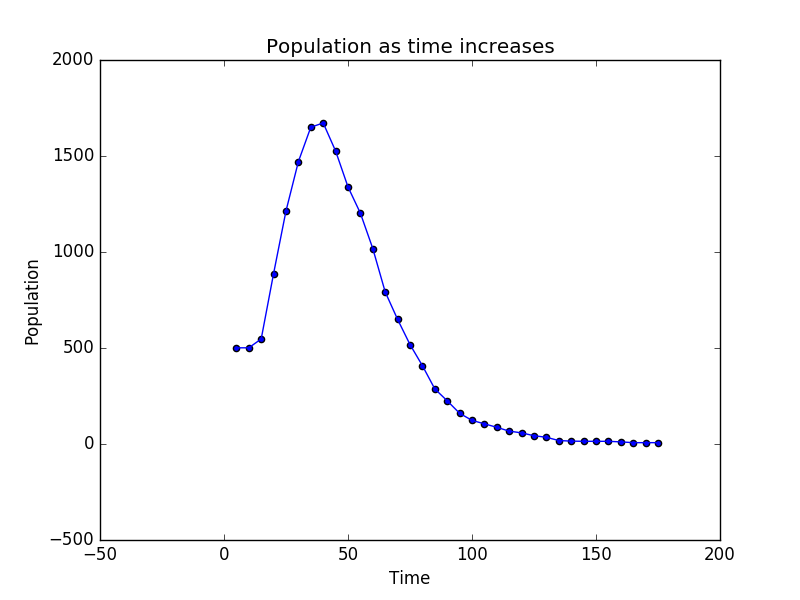
\includegraphics[width=80mm]{Population500noevo.png} \newline
This result appears to show that our agents are not able to keep the population alive. The population appears to peak at around the 45$^{th}$ or 50$^{th}$ time interval, which is around the median age of fertility for the first generation of agents. This pattern did not change significantly when we changed the amount of agents that the simulation started with. We also wanted to see how the simulation would run with evolution. In other words, the parents pass their traits on to their children. Here are the results: \newline
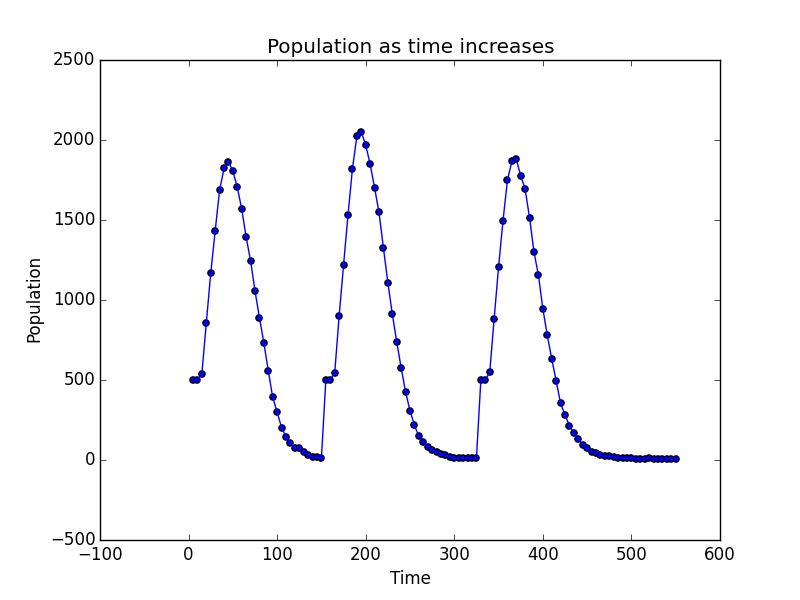
\includegraphics[width=80mm]{Population500.png} \newline
The population died out sooner, but went up to a higher level. \newline
Reproduction seems to stop at the same point as it did without evolution.
This lead us to believe that the first generation of agents were reproducing much more than the later generations. Either the newer generations could not find as many fertile agents, or the food was not replenishing quickly enough. We decided to find out which factor was making it difficult for the agents to reproduce.
\newline
To do this, we kept a counter of the reasons that agents of opposite genders were meeting without reproduction. These reasons included seeing an agent that was already pregnant, not having enough food to support a child, and not being fertile. We also kept track of how many times we checked if a pregnancy was possible. When we did this, we also recorded these levels each time that we checked the population, so that we could see how the increase of these levels accelerates as the simulation progresses. These are the results: \newline
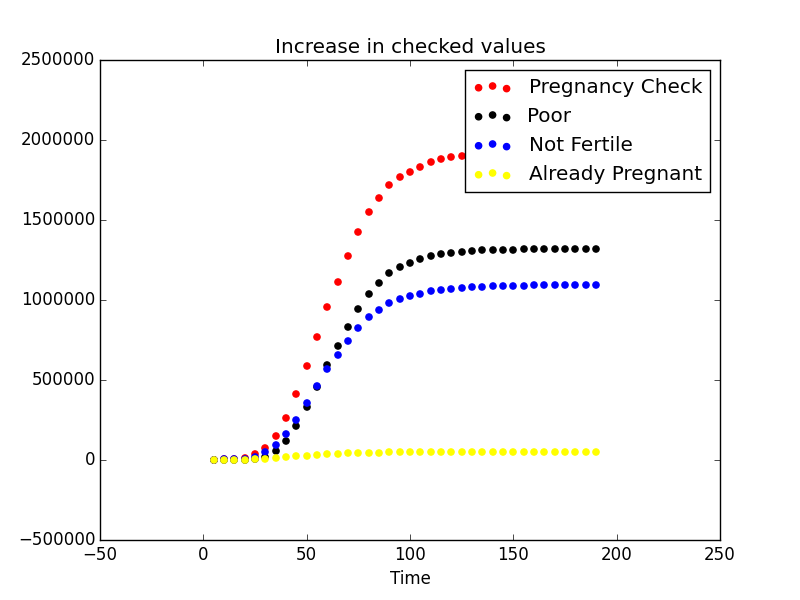
\includegraphics[width=80mm]{factors500.png} \newline
This graph shows that the amount of times that the agents were too poor accelerated more quickly than the amount of times agents were not fertile, so the low amount of resources seems to be doing more damage than fertility, so we doubled the food capacity in each location and made it replenish twice as fast. Here are the results: \newline
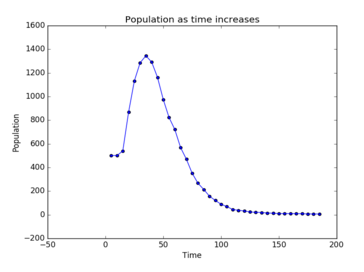
\includegraphics[width=80mm]{FoodCange.PNG} \newline
Increasing the food did not save the population, and even killed them off sooner, so we changed it to its original form and increased the length of fertility. To increase the length of fertility, the men ended fertility at Uniform(50, 60) and women ended at Uniform(60, 70). These are the results: \newline
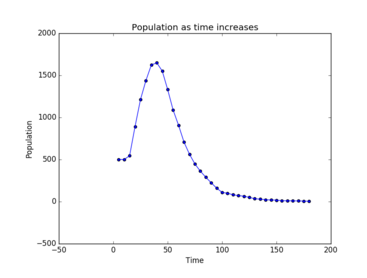
\includegraphics[width=80mm]{FertChange.PNG} \newline
The population lasted longer, but still died out. We then ran a simulation with increased food and fertility. Here are the results: \newline
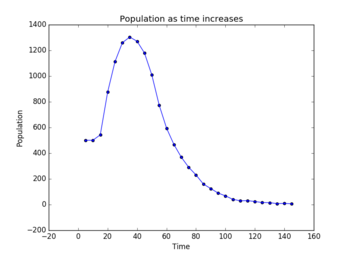
\includegraphics[width=80mm]{both.PNG} \newline
The population still dies out. \newline
\center 
Results and conclusions
\flushleft
When we started the experiments, we ran it without evolution. We saw that the population died out, and its peak was at the middle the point the first generation's fertility (around time = 50). We ran the simulation with evolution and saw that the population died out again, and it peaked at the same point. These results lead us to believe that the later generations were having trouble reproducing, so we decided to find out what was hindering their reproduction. We found that the lack of food that the agents had was doing more damage than the lack of fertility, so we increased the amount of food on the map. This did not save the agents, and actually killed them off sooner, so we tried increasing the length of their fertility. This did not save the agents either, so we increased both of these factors in the same simulation. The population still died out. \newline
In the end, we saw that evolution did have an effect. Even though the agents died off, they did reach a higher point in the size of the population. but the population did not stay alive long enough for us to ask anymore questions. Lack of food and fertility seem to be killing off the population. We have not found a way to save the population, but would like to continue working until we do.









\end{multicols}

\end{document}